\section{Liverpool Life 会议记录}
\label{sec.meeting_record}
作为APR要求的一部分,每位同学作为利物浦的博士生,必须要在一个称作Liverpool-life的系统里,记录自己和导师的会议时间和内容。下面为大家演示一下如何操作。

\begin{enumerate}
    \item 首先进入liverpool-life网站\url{https://liverpool-life.liverpool.ac.uk/},用你的利物浦学号(不是邮箱,更不是西浦学号)和密码登录
    \item 找到PGR Record of Supervisory Meetings,点击View all meetings
    \item 点击Arange new meeting,会弹出窗口,填入日期时间,选择导师(在你后面全部填写完过后,被选中的导师会在他的利物浦邮箱收到邮件)。取消勾选第一个create calendar appointment,否则会在利物浦邮箱的日历里创建一个多半用不上的日程(因为西浦的学生一般都用西浦邮箱对应的日历系统,利物浦的日历系统应该是从来不用的),然后勾选下面的has been pre-agreed。
    \begin{figure}[H]
        \centering
        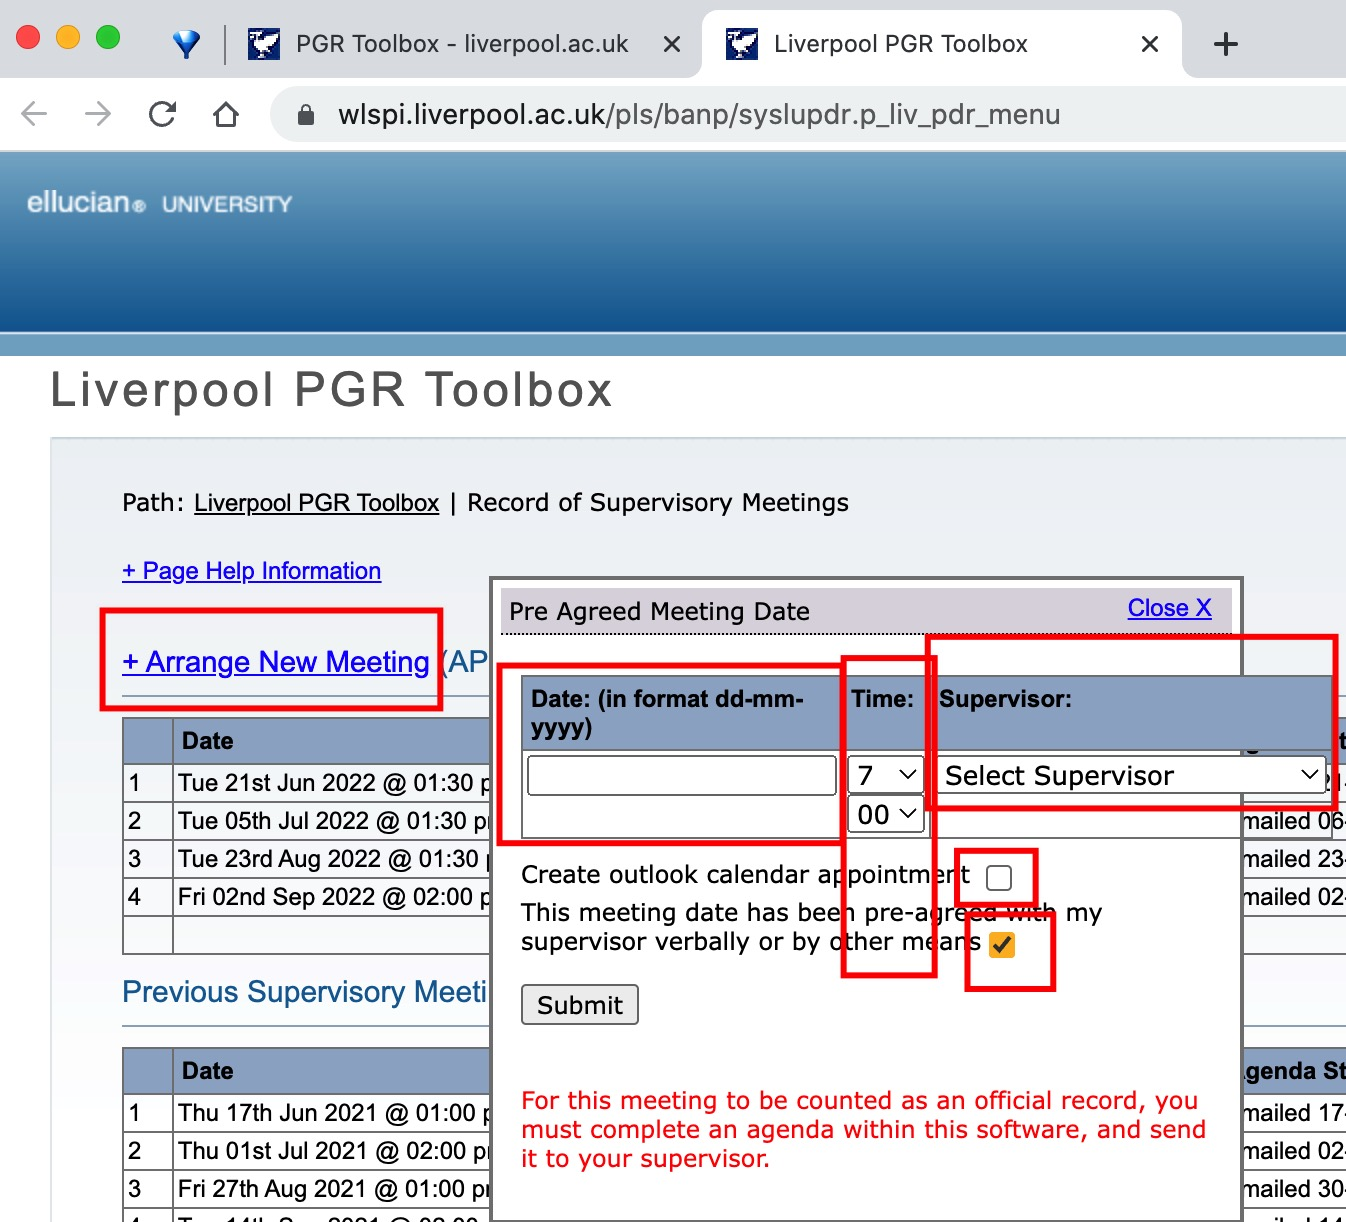
\includegraphics[width=0.5\columnwidth]{author-folder/Kai.Wu/meeting_record_figures/arange_new_meeting.jpg}
    \end{figure}
    \item 然后回忆一下你最近一次跟导师meeting时谈论的内容,填写进度报告(你做了什么)、target(直到下次meeting前打算做什么)、讨论项目
    \begin{figure}[H]
        \centering
        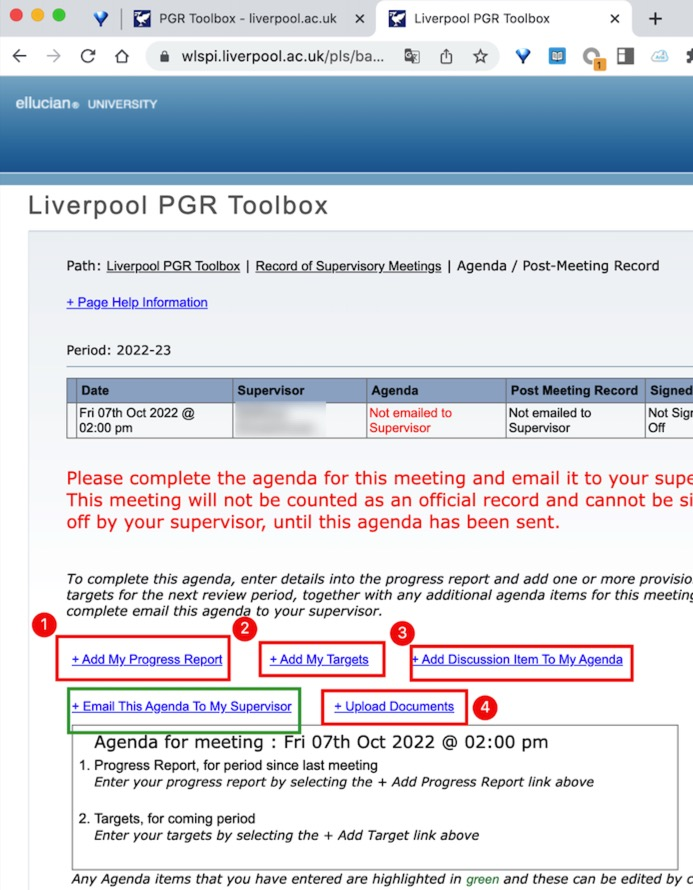
\includegraphics[width=0.5\columnwidth]{author-folder/Kai.Wu/meeting_record_figures/add_items_to_meetings.jpg}
    \end{figure}
    \item 内容不用太多,但也不能太敷衍,毕竟利物浦是要检查的。填完过后,点击email this agenda,然后你和你导师的利物浦邮箱都会收到一封系统自动生成的邮件。
    \begin{figure}[H]
        \centering
        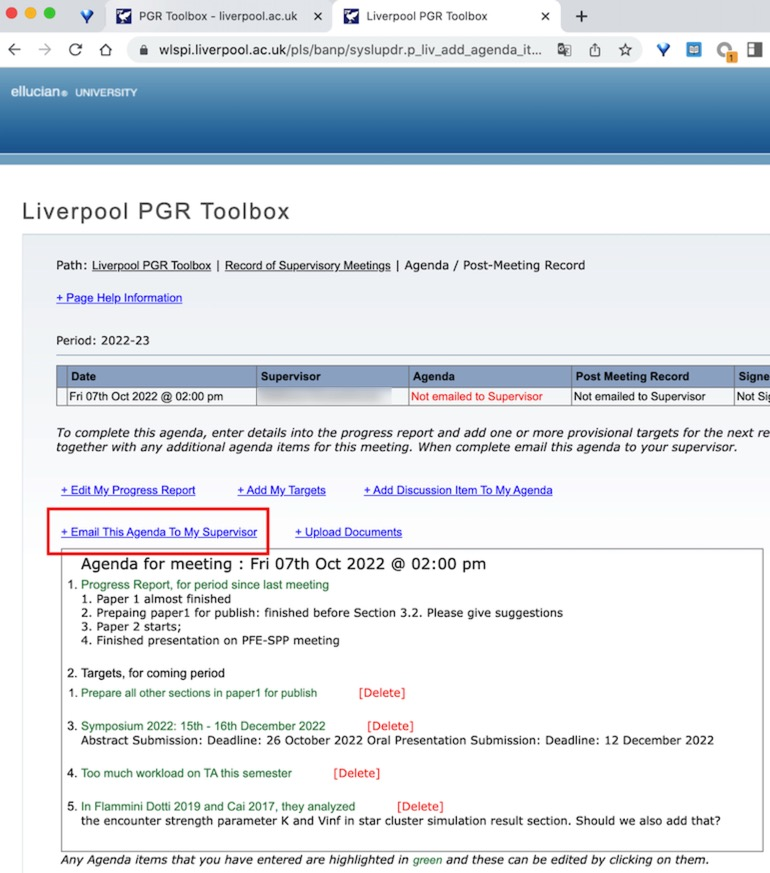
\includegraphics[width=0.5\columnwidth]{author-folder/Kai.Wu/meeting_record_figures/email_to.jpg}
    \end{figure}
    \item 到这里不要着急关闭,还要填一下你们会议中的意见。点击右边的view edit meeting
    \begin{figure}[H]
        \centering
        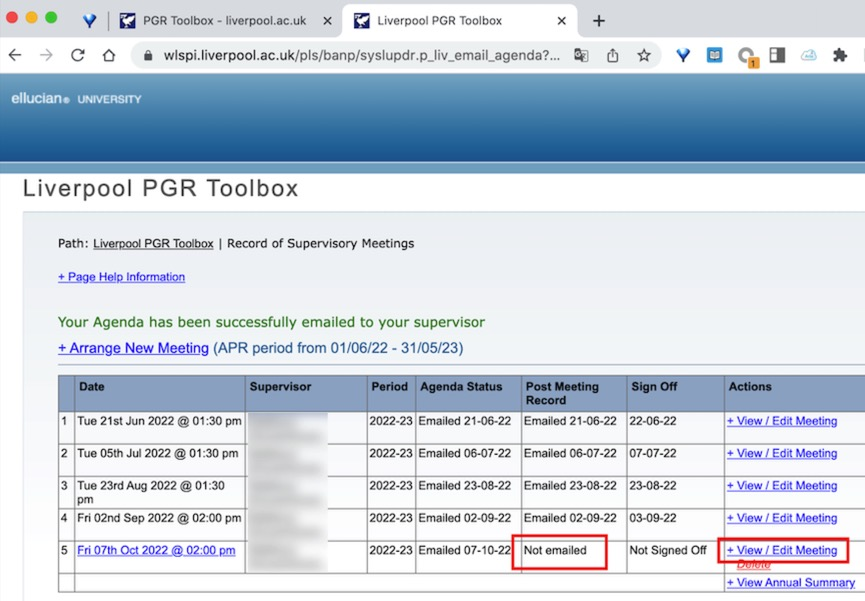
\includegraphics[width=0.5\columnwidth]{author-folder/Kai.Wu/meeting_record_figures/view_edit.jpg}
    \end{figure}
    \item 填入会议中的意见。最后点左上角email,你和导师的利物浦邮箱又会收到一封邮件
    \begin{figure}[H]
        \centering
        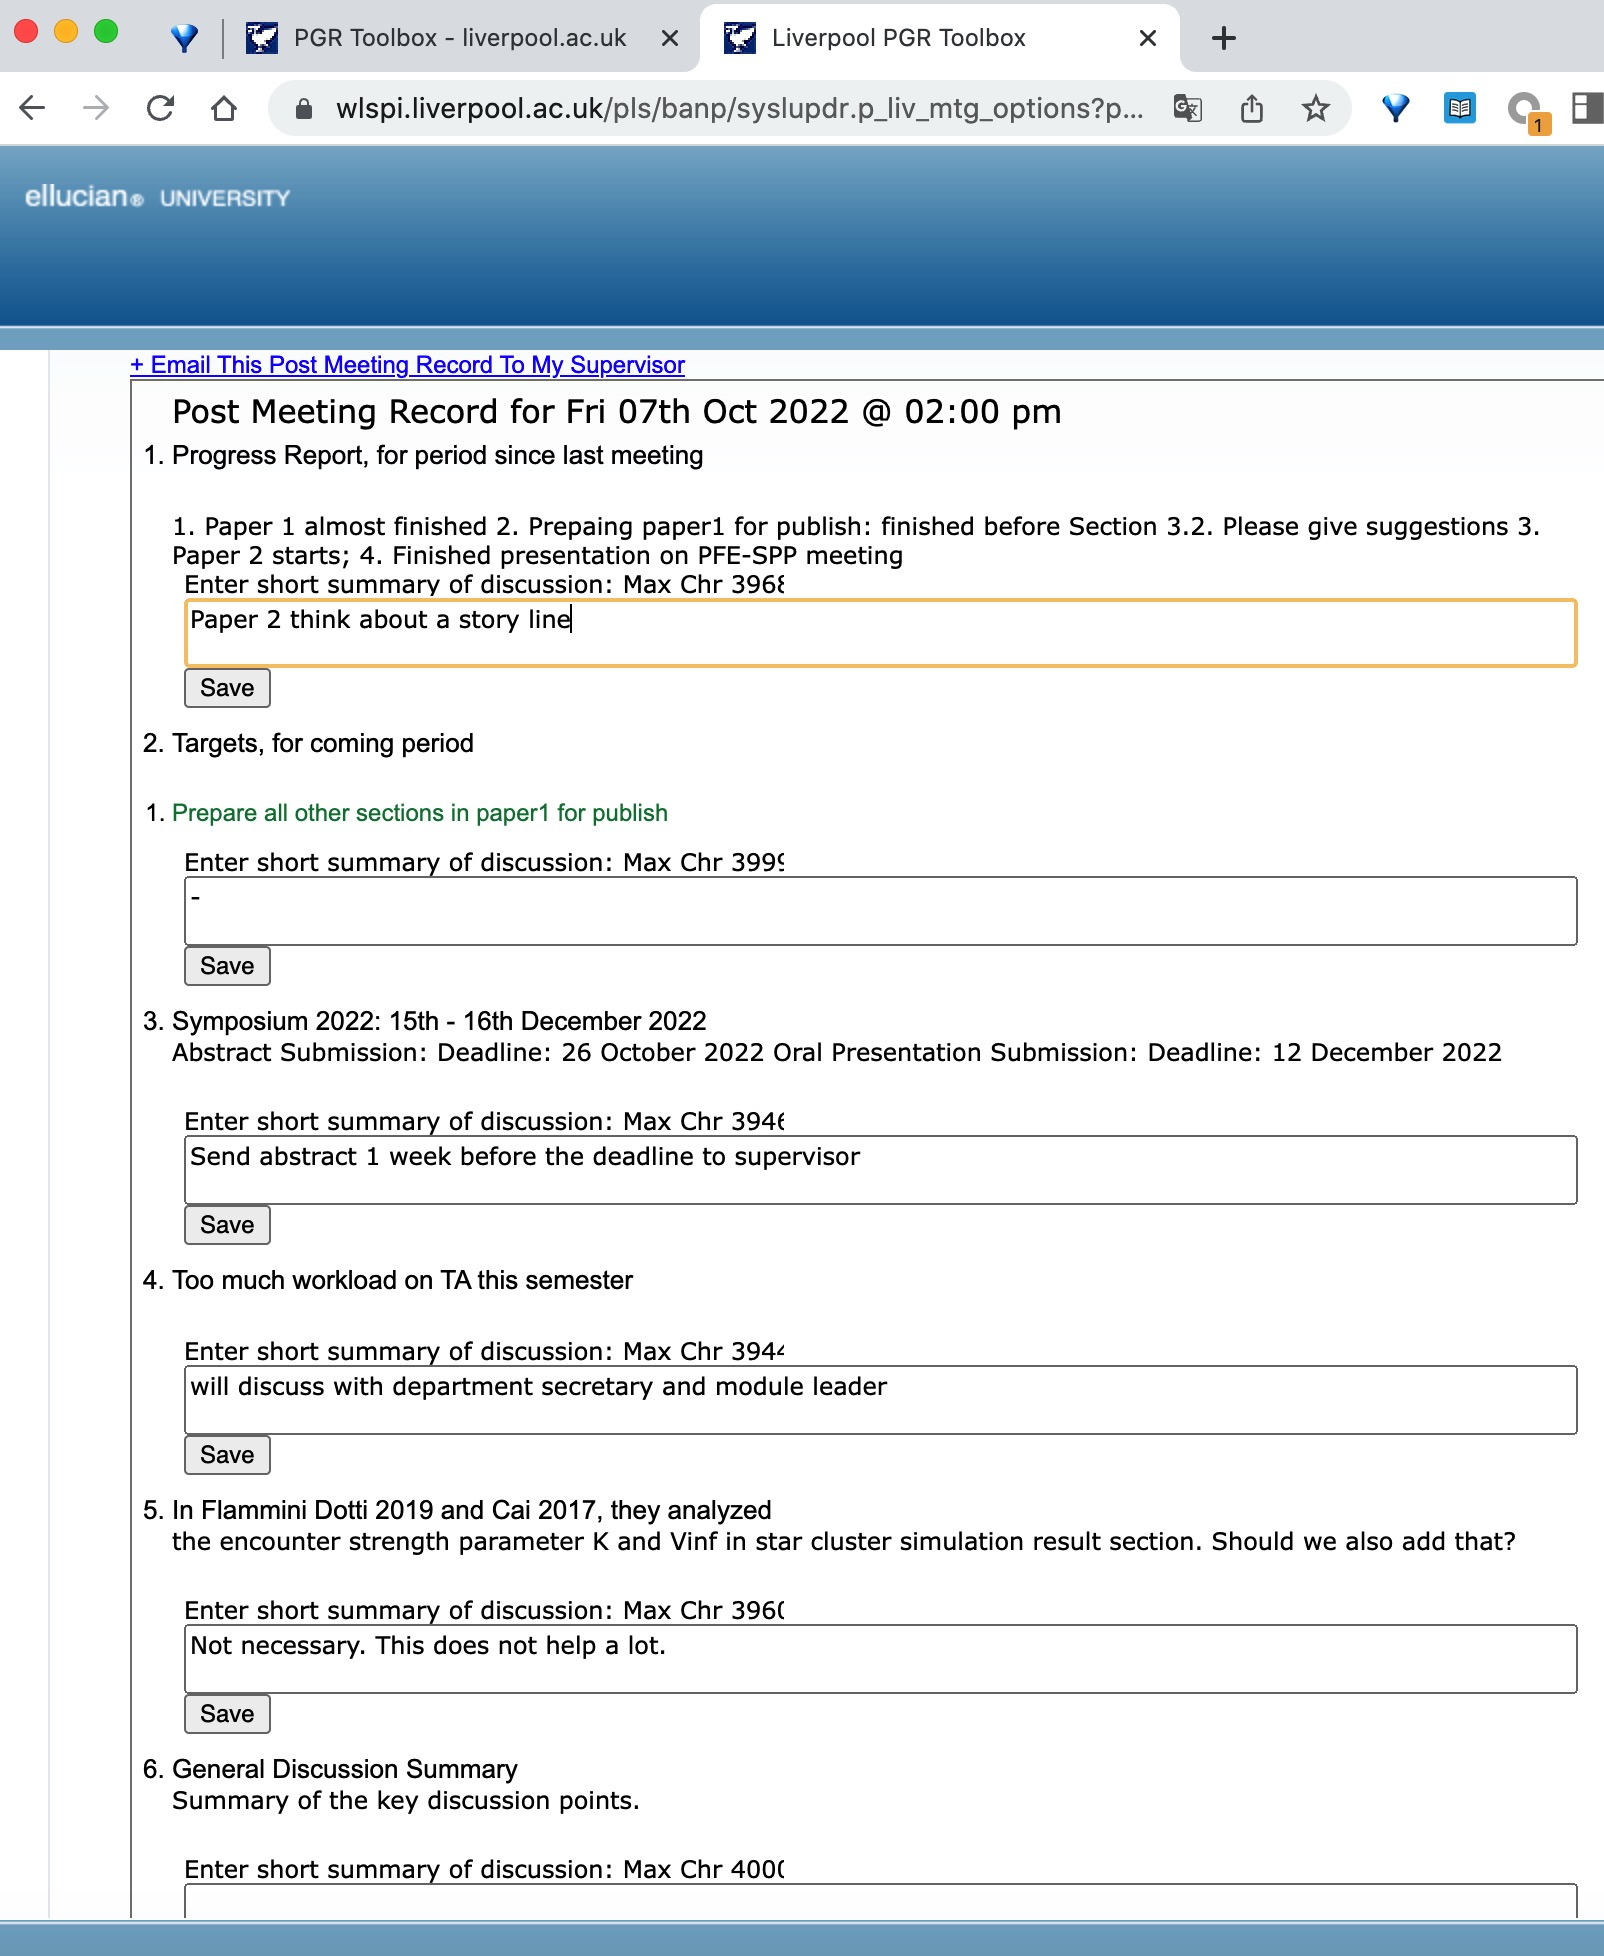
\includegraphics[width=0.5\columnwidth]{author-folder/Kai.Wu/meeting_record_figures/post_meeting.jpg}
    \end{figure}
    % \item 
    %     \begin{minipage}{0.3\textwidth}
    %         由于liverpool life的尿性,建议最后在liverpool life的界面,点击右上角手动登出,否则下次可能很难登录进去
    %     \end{minipage}
    %     \begin{minipage}{0.7\textwidth}
    %         \begin{figure}[H]
    %             \centering
    %             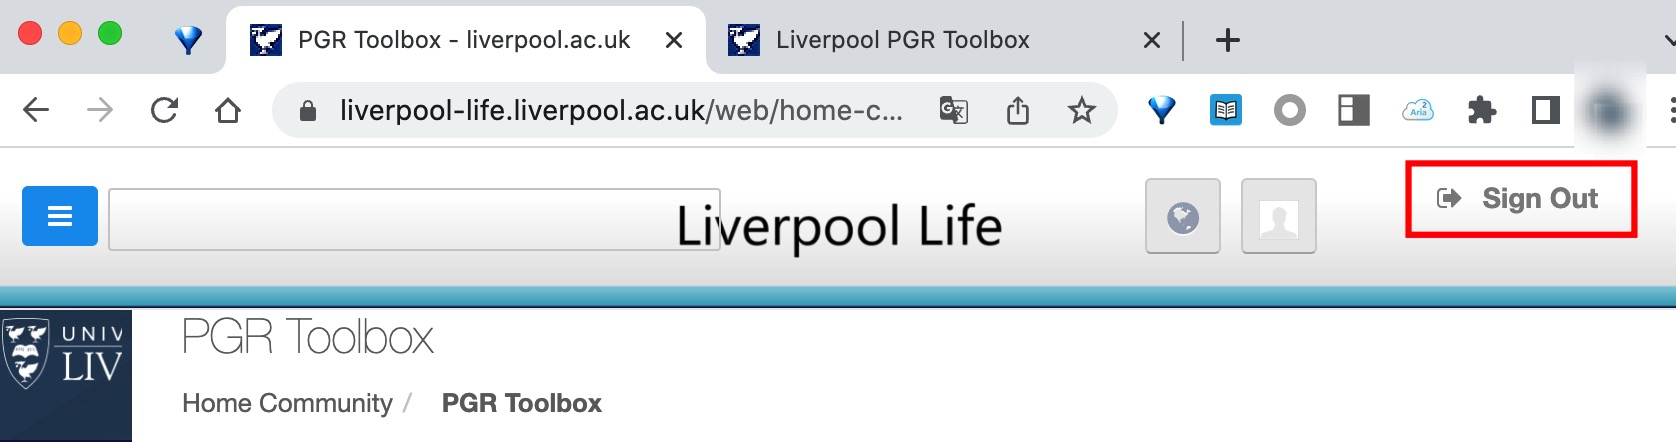
\includegraphics[width=0.9\columnwidth]{author-folder/Kai.Wu/meeting_record_figures/sign_out.jpg}
    %         \end{figure}
    %     \end{minipage}
    % \begin{figure}[H]
    %     \centering
    %     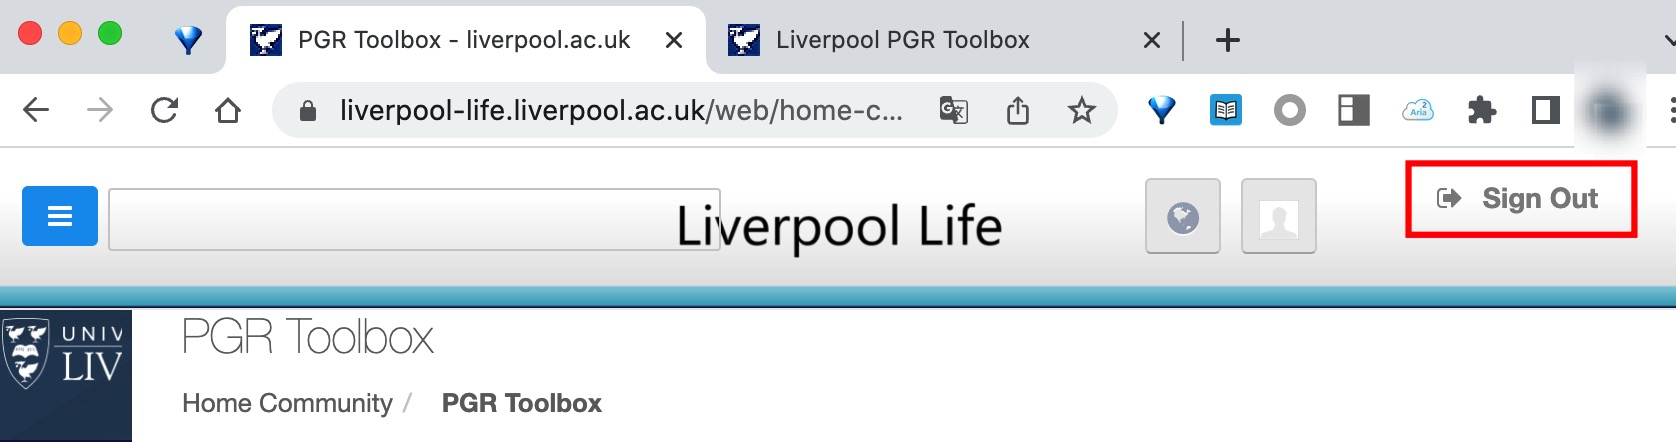
\includegraphics[width=0.5\columnwidth]{author-folder/Kai.Wu/meeting_record_figures/sign_out.jpg}
    % \end{figure}
    \item 到这里你要做的就结束了。你导师需要在他利物浦邮箱收到的邮件里,点击sign off,之后你的利物浦邮箱会收到一封题为 \textit{PGR Supervisor Meeting 5 (Fri 07th Oct 2022 @ 02:00 pm): sign off comments} 的邮件,然后这次meeting record才算全部完成。每年APR之前,必须要每月至少1次的meeting全部sign off。如果你的导师一直没sign off,需要提醒他
\end{enumerate}

\vspace{5mm}
【几个注意事项】
\begin{itemize}
    \item 这个记录最好是每个月填一次。虽然可以补,就是几个月不填然后一口气补半年的,这样是被允许的,但是不规范。我个人的经验里,如果放到APR前夕来补,一来也忘了当年的进度到底是什么,二来APR前夕也很忙。所以,尽量还是按要求每月填一次吧
    \item liverpool life和这个填报网站,经!常!登!不!上!去!因为各种网络和系统的问题,反正即使在西浦校内用wifi和网线都是概率登得上去。据各位同学亲测,一般自己使用科学上网,开全局代理,连通性会好很多,但这些不太合法的方法不能教给大家,也万万不能在微信、QQ里讨论,否则会封号、炸群。不会科学上网的同学,更是要尽量早填报,否则到deadline登不上去就更着急。
\end{itemize}

\begin{flushright}
    (2022年10月10日 by \Wu)
    \end{flushright}